\documentclass[../main.tex]{subfiles}
\begin{document}
\graphicspath{{../imagenes/fourier/applet/}}

\section{Fourier Applet}
Este programa demuestra la serie de Fourier, que es un método para expresar
una función periódica arbitraria como una suma de términos. 

Para seleccionar una función puede presionar uno de los siguientes botones:
Sine, Cosine, Triangle, Sawtooth, Square, Noise, Phase Shift, Clip,
Resample, Quantize, Rectify, Full Rectify, High - Pass Filter, Clear.

También se puede generar una señal a gusto arrastrando el mouse o dedo, dependiendo
de que dispositivo se use, para dibujar una señal, también se mostrará las armónicas
de la señal que se dibujó. 

Debajo de los botones de funciones existen dos barras para interactuar.
Una para modificar la cantidad de armónicos “Number of terms” y otra para
cambiar la frecuencia “Playing Frecuency”. 

En las señales periódicas y que se le pueda aplicar series de fourier los
vectores varían y los armónicos se transforman en una gráfica de
$+\infty$ a $-\infty$. Para eso:

\begin{figure}[H]
	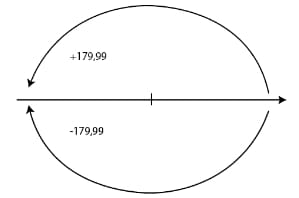
\includegraphics[width=0.6\textwidth]{imagen1.png}
	\centering
\end{figure}

Esto hace que los armónicos sólo puedan variar hasta $\pi$ (179,99) a -$\pi$ (-179,99).
\subsection{Las funciones}
	\subsubsection{Sinusoidal}
	La señal senoidal está conformada de dos botones: el Sine y el Cosine
	\subsubsection{Sine}
	\begin{figure}[H]
		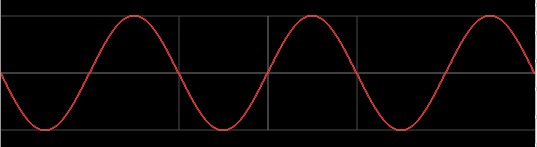
\includegraphics[width= 0.6 \textwidth]{imagen2.png}
		\centering
	\end{figure}

	\subsubsection{Cosine}
	\begin{figure}[H]
		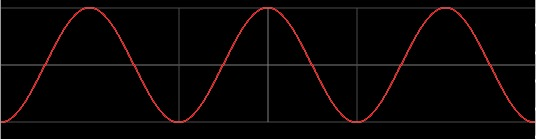
\includegraphics[width= 0.6 \textwidth]{imagen3.png}
		\centering
	\end{figure}
	Ambas señales tienen una forma muy similar, lo único que cambiaría sería que el 
	coseno(Cosine) está desplazado hacia la izquierda respecto al seno(Sine) 
	en un cuarto de ciclo. Las ondas senoidales son las funciones de seno y de coseno.
	En el eje vertical se coloca la magnitud en cuestión, mientras que en el
	eje horizontal se ubica el tiempo

	\subsubsection{Triange}
	\begin{figure}[H]
		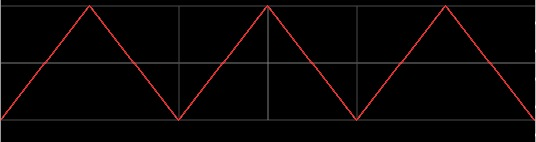
\includegraphics[width= 0.6 \textwidth]{imagen4.png}
		\centering
	\end{figure}
	Es una función que tiene una sintonía par porque se compone únicamente de cos().

	\subsubsection{Sawtooth}
	\begin{figure}[H]
		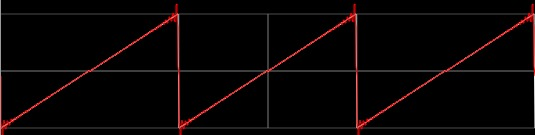
\includegraphics[width= 0.6 \textwidth]{imagen5.png}
		\centering
	\end{figure}
	Es una función que tiene una sintonía impar porque se compone únicamente de sen().

	\subsubsection{Square}
	\begin{figure}[H]
		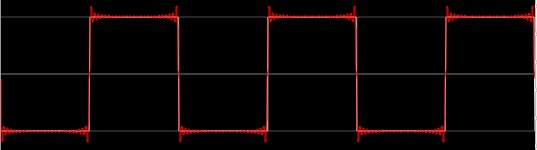
\includegraphics[width= 0.6 \textwidth]{imagen6.png}
		\centering
	\end{figure}
	La discontinuidad en una onda cuadrada y en el cambio abrupto que 
	parece tener dos valores de x en el mismo momento
	\begin{figure}[H]
		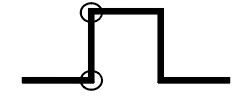
\includegraphics[width= 0.3 \textwidth]{imagen7.png}
	\end{figure}
	Se aplica una discontinuidad (limites matematicos).
	\begin{figure}[H]
		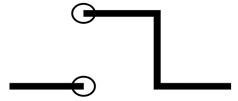
\includegraphics[width= 0.3 \textwidth]{imagen8.png}
	\end{figure}
	Por lo que en realidad no son rectas porque dejarían de ser una función matemática.

	\subsubsection{Noise}
	\begin{figure}[H]
		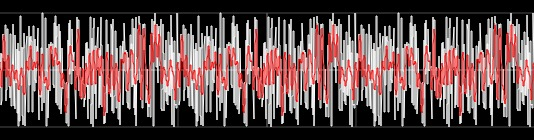
\includegraphics[width=0.6\textwidth]{imagen9.png}
		\centering
	\end{figure}
	El ruido se ocasiona cuando se produce un campo magnético alrededor de los conductores.
	Un campo magnético es la explicación matemática de la influencia magnética de
	las corrientes eléctricas. Una corriente eléctrica es el movimiento de los electrones.

	\subsubsection{Phase Shift}
	Hace un desfase en la señal.

	\subsubsection{Clip}
	Acorta la señal hasta hacerla una onda cuadrada.

	\subsubsection{Resample}
	Va reordenando los armónicos de la señal para convertirla de a poco en una onda cuadrada.\\
	Por ejemplo:\\
	Para una señal dientes de sierra.
	\begin{figure}[H]
		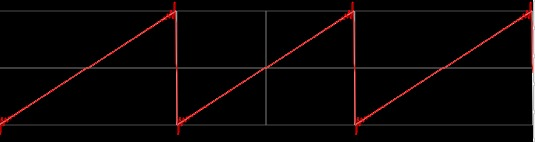
\includegraphics[width= 0.6 \textwidth]{imagen10.png}
		\centering
	\end{figure}
	\begin{figure}[H]
		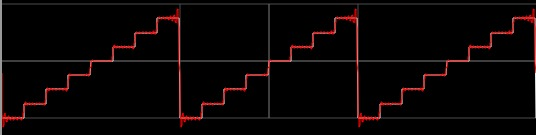
\includegraphics[width= 0.6 \textwidth]{imagen11.png}
		\centering
	\end{figure}
	\begin{figure}[H]
		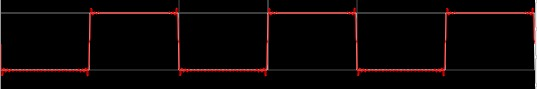
\includegraphics[width= 0.6 \textwidth]{imagen12.png}
		\centering
	\end{figure}

	\subsubsection{Quantize}
	Mueve los armónicos para hacer una señal más cuadrada de dicha onda.\\
	Por ejemplo:\\
	Para una señal dientes de sierra.
	\begin{figure}[H]
		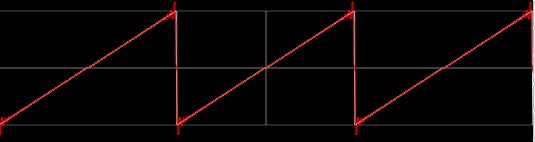
\includegraphics[width= 0.6 \textwidth]{imagen13.png}
		\centering
	\end{figure}
	\begin{figure}[H]
		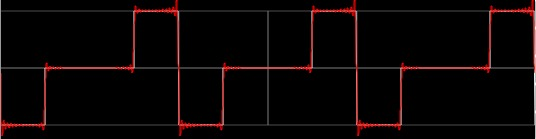
\includegraphics[width= 0.6 \textwidth]{imagen14.png}
		\centering
	\end{figure}
	\textbf{Resample vs Quantize}
	\begin{itemize}
		\item Si la señal es sine o triangle:\\ 
			Resample ordena las armónica de sines 
			y cosines, mientras que Quantize solo ordena las de sine. 

		\item	Si la señal es cosine o Sawtooth:\\ 
			Quantize ordena las armónica de sines y cosines.
			Mientras que resample solo ordena las de sine. 

		\item	Si la función es Square:\\
			Ni resample ni Quantize ordenan alguna armónica. 

		\item	Si es un Noise:\\
			Tanto Quantize como Resample ordenan las armónicas de sine y cosine.
			Sim embargo, en Resample el sonido se vuelve una señal cuadrada.

		\item Si es Quantize:\\
			mantiene su forma de ruido, pero tiene una forma más ``recta''
	\end{itemize}
	\subsubsection{Rectify}
	Rectifica la parte negativa de la señal y la pone en 0.

	\subsubsection{Full Rectify}
	Rectifica la parte negativa de la señal y la pone igual que la parte positiva.

	\subsubsection{High-Pass Filter}
	Es un filtro pasa altos.

	\subsubsection{Clear}
	Limpia la señal.


	\subsubsection{Number of Terms}
	Una barra que se puede arrastrar usando el mouse o tocando las flechitas que están
	a los costados. Su función es aumentar o reducir la cantidad de armónicos de forma
	manual. 

	Esto no afecta directamente a la forma de la señal.
	\begin{figure}[H]
		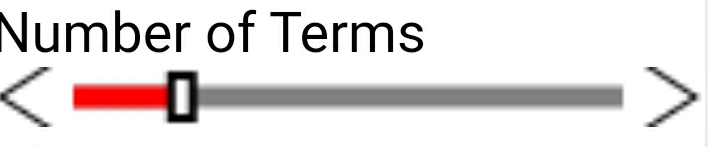
\includegraphics[width= 0.6 \textwidth]{imagen15.jpg}
		\centering
	\end{figure}
	En la imagen se puede ver una función seno (sine) con la cantidad respectiva de armónicos que la barra representa.

	\begin{figure}[H]
		%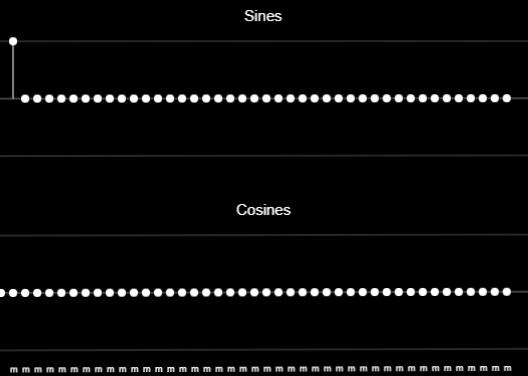
\includegraphics[width= 0.6 \textwidth]{imagen16.jpg}
		\centering
	\end{figure}

	Los armónicos que se encuentran en esa zona se pueden “levantar” o “bajar” afectando
	a la forma de la señal. Dependiendo de si el armónico es uno de los primeros o uno de
	los últimos, la señal se verá deformada en mayor o menor medida.

	El primer armónico del coseno (cosines) no deforma la señal, si no que cambia la
	posición de la señal, elevandola por encima o debajo del cero. 
	\begin{figure}[H]
		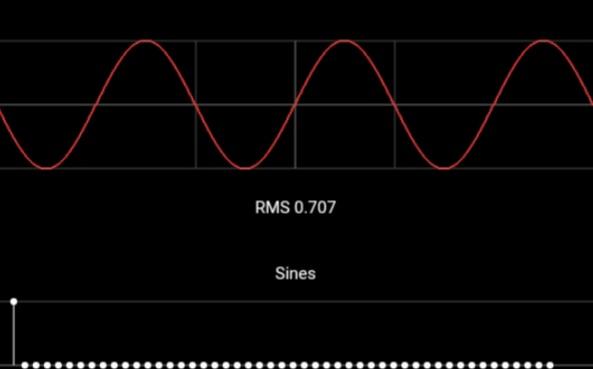
\includegraphics[width= 0.6 \textwidth]{imagen17.jpg}
		\centering
	\end{figure}
	\begin{figure}[H]
		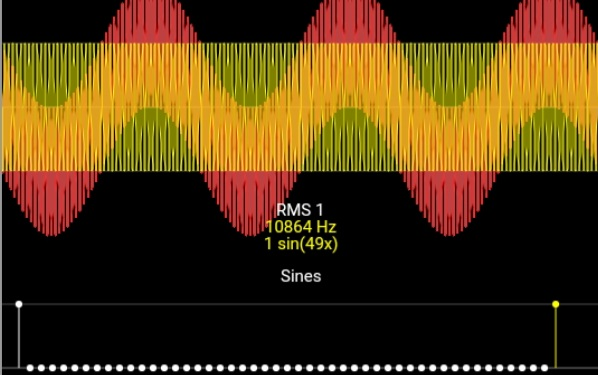
\includegraphics[width= 0.6 \textwidth]{imagen18.jpg}
		\centering
	\end{figure}
	Como ejemplo tenemos estas dos imágenes:
	En la primera imagen se puede ver una señal sine y en la segunda imagen se puede ver
	la misma señal con el último armónico “levantado” deformando bastante la señal. 

	Las funciones “Resample” y “Quantize” se encargan de organizar los armónicos
	automáticamente para hacer que la señal se vea más “cuadrada”.

	\subsubsection{Playing Frequency}
	Una barra que se puede arrastrar usando el mouse o tocando las flechitas que están a
	los costados. Su función es aumentar o reducir la frecuencia de la señal. 
	Esta barra sirve para escuchar la señal usando el botón ``Sound''
	(verificar el volumen del dispositivo antes de activarlo). 
	\begin{figure}[H]
		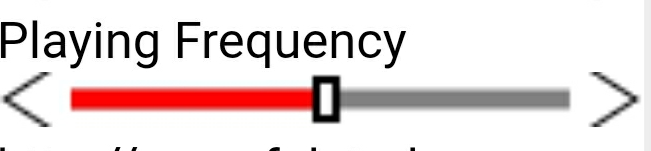
\includegraphics[width= 0.6 \textwidth]{imagen19.jpg}
		\centering
	\end{figure}
\end{document}
